\subsection{Petri net editor}
\label{sec:sf-petrinet}
\writer{Albert}

The Petri net editor is a component that will extend the features provided by the \textit{ePNK}, in order to fulfil the requirements of the project. The extended features include \textit{Input Places} and the definition of links between geometry and animation components.

\subsubsection{Functional Requirements}

\begin{enumerate}
	\item The Petri net editor \textbf{shall} allow the user to create, edit and delete Places.
	\item The Petri net editor \textbf{shall} allow the user to create, edit and delete Tokens inside Places.
	\item The Petri net editor \textbf{shall} allow the user to create, edit and delete Transitions.
	\item The Petri net editor \textbf{shall} allow the user to create, edit and delete Arcs. An arc \textbf{shall} connect a Place to a Transition or vice versa.
	\item The Petri net editor \textbf{shall} allow the user to define a Geometry label to a Place.
	\item The Petri net editor \textbf{shall} allow the user to define an Appearance label to a Place.
	\item The Petri net editor \textbf{shall} allow the user to define an Input Place label to a Place.
	\item The Petri net editor \textbf{shall} allow the user to define an Animation label to a Place.
	\item The Petri net editor \textbf{shall} allow the user to save and load a Petri net model.
	\item The Petri net editor \textbf{shall} create a Petri net file in a format that can be read by the Simulator.
	\item It \textbf{would be nice} that the Petri net editor allowed the user to undo and redo actions.
	\item It \textbf{would be nice} that the Petri net editor allowed the user to copy and paste.
\end{enumerate}

\subsubsection{Use cases}

The features are shown in Figure~\ref{fig:use-cases-petri-net-editor}.

\begin{figure}[htp]
\begin{center}
  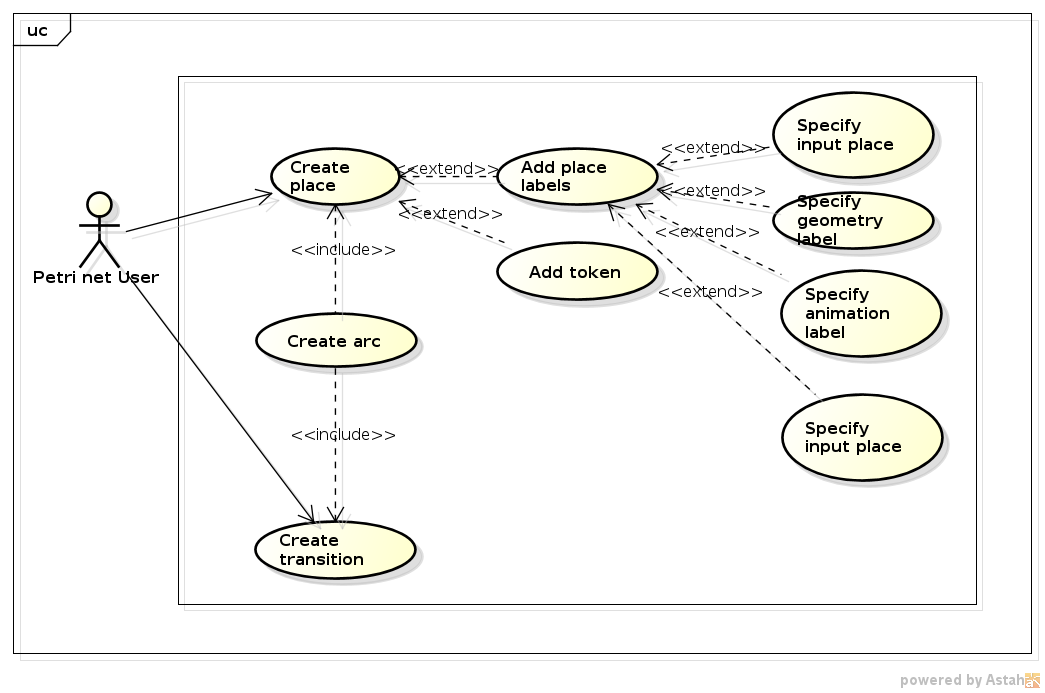
\includegraphics[width=0.8\textwidth]{image/uc-petri-net.png}
  \caption{Use cases for the Petri net Editor}
  \label{fig:use-cases-petri-net-editor}
\end{center}
\end{figure}